\documentclass[10pt, a4paper]{report}
\usepackage[utf8]{inputenc}
\usepackage{lscape}   % Make a page in landscape format \begin{landscape}
\usepackage{colortbl} % To color table cells
\usepackage{color} % Able to change textcolor
\usepackage[table]{xcolor}
\usepackage{longtable}
\usepackage{graphicx} % Able to add pictures
\usepackage{parskip}  % Separate paragraphs with a blank line
                      % rather than using indentation
\usepackage{hyperref} % Support for hyperlinks
\usepackage[protrusion=true,expansion=true]{microtype} % Improve justification
\usepackage{subfigure}
\usepackage{hyperref}
\usepackage{caption}
\usepackage{float}
\usepackage{afterpage}
\usepackage{lipsum}
\usepackage{wrapfig}
\usepackage{enumerate}
\usepackage{natbib}
\usepackage{todonotes}
\usepackage{mdwlist}
\usepackage{array}
\usepackage{listings}

\definecolor{lightgray}{rgb}{.9,.9,.9}
\definecolor{darkgray}{rgb}{.4,.4,.4}
\definecolor{purple}{rgb}{0.65, 0.12, 0.82}

\lstdefinelanguage{JavaScript}{
  keywords={typeof, new, true, false, catch, function, return, null, catch, switch, var, if, in, while, do, else, case, break},
  keywordstyle=\color{blue}\bfseries,
  ndkeywords={class, export, boolean, throw, implements, import, this},
  ndkeywordstyle=\color{darkgray}\bfseries,
  identifierstyle=\color{black},
  sensitive=false,
  comment=[l]{//},
  morecomment=[s]{/*}{*/},
  commentstyle=\color{purple}\ttfamily,
  stringstyle=\color{red}\ttfamily,
  morestring=[b]',
  morestring=[b]"
}

\lstset{
   language=JavaScript,
   backgroundcolor=\color{lightgray},
   extendedchars=true,
   basicstyle=\footnotesize\ttfamily,
   showstringspaces=false,
   showspaces=false,
   numbers=left,
   numberstyle=\footnotesize,
   numbersep=9pt,
   tabsize=2,
   breaklines=true,
   showtabs=false,
   captionpos=b
}


\hypersetup{%
    pdfborder = {0 0 0}
}

\begin{document}
	
	\pagenumbering{arabic}
	\begin{titlepage}
\begin{center}

{\Huge Project Thesis} \\[1.0cm]
{\Large Norwegian University of Science and Technology}\\[4.0cm]


\end{center}
\end{titlepage}\clearpage \thispagestyle{empty}
	\section*{Abstract}
  
  Since the first proposal for a graphical password around 1999, a variety number of graphical password schemes have been proposed. The proposed graphical password schemes were motivated by the promise of improved password memorability and thus usability, while at the same time trying increase the security.  Psychology studies have recognized that the human brain have a superior memory for recognizing and recalling visual information rather than recognizing and recalling verbal or textual information. Graphical passwords seems as a good replacement of text-based authentication. 

  The motivation for this thesis started by observing the shortcomings with text-based authentication, where people tend to obtain bad habits because of the difficulty of remembering the textual information. People therefore tend to create easily guessed passwords. Password sharing and password reuse are also some of the know habits that people obtain by using text-based passwords. When looking at mobile devices, text-based passwords are not easily typed on a mobile screen. Graphical passwords do not only seem as a good replacement of text-based passwords, but also look like a great authentication method for mobile devices because of the easily interaction with graphical elements on a small touch screen. 

  Android Unlock Patterns is one of the graphical password schemes with an commercial success on mobile devices. The only large-scale study that have conducted quantified the security of peoples choice in patterns. This study aims to take the analysis of people's choice in Android Unlock Patterns a step further by including the human properties that may impact the user's choice in graphical passwords. I believe that graphical passwords are more than just pictures and graphical objects.

  In this thesis there is conducted a literature review of graphical passwords. There is also created a proposal for a research design for further continuation of this work. The research design contains a research strategy, as well as a prototype for data collection. 

  \clearpage \thispagestyle{empty} \cleardoublepage 
	\tableofcontents \clearpage \thispagestyle{empty} \cleardoublepage 

	\listoffigures
	\listoftables
	
	%Chapter 1 - Introduction
	\setcounter{page}{1}
	\chapter{Introduction}

  This chapter is an introduction to the research project. Section~\ref{sec:background} is the background and motivation for conducting this research. Section~\ref{sec:researchquestions} includes the research questions to be answered in this report. Section~\ref{sec:deliverables} is a description of what will be the deliverables of this research.
  The methods used in this project is described in Section~\ref{sec:methods}. The last section is an overview of the structure according to the chapters included in this report. 

  \clearpage
  \section{Background and Motivation} \label{sec:background}
  In today's society, people tend to spend much time on their mobile devices. Mobile devices are not just tool for communication, but also an essential tool for everyday tasks like reading mail, pay our bills, and keeping up with our social life. Our whole life is contained in one device. When such a small device is so central to our daily lives, it makes it vulnerable.

  Passwords are human-chosen secrets that are connected to you as a person. When creating a password, people tend to create a password that is an association to something they know or recognize; passwords are more than just words and numbers. Because of the shortcomings with text-based passwords \cite{UnixPasswords}, there is an increased interest in graphical passwords. The interest in graphical passwords started by the assumption that pictures are easier to remember and more secure than words and numbers \cite{DeAngeli}.

  The motivation for this thesis began by observing the shortcomings with the text-based authentication. Password reuse is one of the known password habits among users because the human limitation to remembering text-based password. Some users also make simple or meaningful password that are easier to remember, making their passwords vulnerable to attacks. Graphical passwords look like a promising alternative to text-based passwords, as it supports users to remember and make more complex passwords, offering better usability and higher security. As mobile devices play a significant role in our everyday life, it makes it interesting target device. Security on mobile devices has changed during the past years. The history of locking mechanisms was often a solution solely to prevent accidental use, while current mobile phones require protection in order to secure the potentially vast amount of private data that we keep on our mobile devices. The situation of our rapid use of mobile devices, as well as it well-suited platform for graphical password, makes authentication on mobile devices an interesting field of study.

  Google's Android platform released the functionality for the Android Unlock Pattern in 2008. The Android Unlock Pattern is a graphical authentication scheme that enables the users to connect dots as their password. Since its release, there have been much discussion of its security, but few researchers have conducted scientific research on the Android Unlock Pattern. The problem is not just the theoretical password space, but rather the password space in practice. In 2013, a research group conducted the first large-scale user study on the Android Unlock Patterns \cite{Uellenbeck}. The Android Unlock pattern is a screen lock mechanism for the Android mobile operating system. The outcome of the research was an analysis of 2900 user-selected patterns. They found bias in the pattern making process claiming that the scheme are less secure than its stated theoretical password space.

  The aim of this research is to look further into how different user types select their Android Unlock Patterns. This takes previous research a step further by including the human properties that may impact the user's choice in graphical passwords. I believe that graphical passwords are more than just pictures and graphical objects. This thesis is the first phase of my research and will be continued in my master thesis in the following spring.

  \section{Research Questions} \label{sec:researchquestions}
    
  This section contains three research questions to be answered in this research project. They are created based on the introduction and background in Section~\ref{sec:background}. This thesis is the first phase of my research and will be a supporting work for my master thesis that will be a continuation of this project.

  {\bf $RQ1$: What is the status of current research on graphical passwords?} \\
  To answer this research question, there will be conducted a literature review, and will give an overview of the research that is published in the field of graphical passwords. The goal is to find a gap in the research that can be answered in my master thesis as a continuation of this work.

  {\bf $RQ2$: What human properties may affect our choice of graphical passwords on mobile devices?}\\
  My motivation is to find human properties that may impact user's choice in graphical passwords on mobile devices. To answer this, there need to be conducted a review of human properties that describe different user types.

  {\bf $RQ3$: How are we able to collect user-chosen patterns set by various user types?}
  To be able to analyze user-chosen patterns set by different user types, we need to design a prototype for data collection. Collecting user-chosen passwords is not easy to do because people do not give away their passwords easily. When collecting graphical passwords, there is no data source available. It should also be considered how to reach people quickly in order to get a large sample size that can provide statistical significant results in an analysis.

  \section{Deliverables} \label{sec:deliverables}

  There will be three main deliverables in this thesis.

  {\bf Literature review}: The first part of this research is a literature review on graphical passwords. A literature review is providing the information needed to decide on the main research hypothesis for my master thesis, and the aim is to fill the gap in research on graphical passwords on mobile devices.

  {\bf Research design}: The gap found in the literature review will result in a problem domain to be worked in my master thesis. To be able to continue with this work, the research design for next semester will a deliverable of this work. The research design is mainly a detailed description of the research strategy and data collection method.

  {\bf Prototype for data collection}: Research on passwords is not easy to conduct because of the nature of passwords. Passwords should remain a secret for the user, and as we have learned, we should not share our password due to security concerns. Research on text-based passwords is often based on leaked password on the web. When analyzing graphical passwords on mobile devices, there is no such data source available. The prototype can provide insight into a new way of solving the problem of collecting user chosen passwords from mobile devices. This can provide knowledge for future research on graphical passwords on mobile devices. The deliverable will be a suggested prototype for data collection and the data that is desired to collect besides the passwords.

  \section{Methods} \label{sec:methods}

  This section will give a description of the methods used in this research project. 

    \subsection{Research Process} \label{sec:methodresearchprocess}

    Throughout this thesis, the research process illustrated in Figure~\ref{fig:researchProcess1} will be used as a basis for the elaboration of how to conduct the research in my master thesis. The research process is a framework for researching information systems and computing \cite{empiriske}. The only part of the research process that is carried out in this thesis is the background and motivation, as well as the literature review.

      \begin{figure}[H]
        \centering
        \includegraphics[scale=0.18]{pics/ResearchProcess.png}
        \caption[Research process]{Research Process \cite{empiriske}}
        \label{fig:researchProcess1}
      \end{figure}

    Experiences and motivation is a description of why to conduct the research. A literature review is a review of published research in the selected area of study. By studying the literature, it is given the ability to synthesize it into a coherence account that justifies the chosen research and places it in the context. The literature review should help provide a conceptual framework, that is, the an explicit way of to how I structure the thinking about the research topic and the process undertaking. The conceptual framework includes different factors that comprise the selected topic, the way of thinking about the subject and the way of tackling the research questions. A research strategy is the overall approach to answering the overall hypothesis and research questions. There are six different research strategies: survey, design and creation, experiment, case study, action research, and ethnography. A data generation method how to produce empirical data or evidence. There are four data generation methods: interviews, observation, questionnaire, and documents. Data can either be qualitative or quantitative. 

    \subsection{Literature Review}\label{sec:methodliteraturereview}

    A literature review is often used for two main purposes. {\it First}, by exploring the research, it is useful to look for a suitable research idea and discover relevant material about any possible research topics. {\it Second}, the second part often begin once a research topic is chosen, where the aim is to gather and present evidence to support that the research can produce new knowledge.

    There is a broad range of sources to be used in the literature review, for example, books, journal articles, and conference papers. Books are often based on well know facts with a broad scope. Journal articles and conference papers are more exploratory and are useful for finding information on the current thinking and research in the area. All published journals and conference proceedings needs to be reviewed carefully. It is important to use the sources that is considered to publish quality research and that they provide sufficient quality control on the published research. Some highly rated journals in information systems and computing is: ACM \cite{ACM}, IEEE \cite{IEEE}, and Springer \cite{Springer}. When using conference papers, it can often be useful to read something about their review procedures and their quality requirements. Besides the publication source, it can be helpful to look at the number of citations used. If a research paper has many citations, it may be an indication of it quality.

    When reviewing the literature, it would be too time consuming to read all the papers from the start to the end. To be able to select relevant research, it is preferable to look at the abstract first that should include information about the research motivation, the methods used, as well as the results. If the abstract were promising, I would continue reading the results, and methods used. If the research is very interesting, it might be valuable to read the whole publication.

    Before searching for relevant literature, it is important to define keywords that can narrow the search down to obtain information that is relevant according to the research that is being conducted. The keywords can be combined when searching in different digital libraries.

    When relevant literature is found, it is important to set a list of quality criteria that until now have been discussed.
    The selected quality criteria that are chosen is listed in Table~\ref{tab:QualityCriteria}.

      \begin{table}[H]
        \centering
        \begin{tabular}{| l | p{10cm} |}
          \hline
          {\bf \#} & {\bf Quality Criteria} \\ \hline
          QC 1 & The research is published in a known digital library, journal or conference\\ \hline
          QC 2 & There is a clear statement of the aim of the research\\ \hline
          QC 3 & The study is cited by other researchers\\ \hline
          QC 4 & There is a clear description of the method used in the study\\ \hline
          QC 5 & If the research includes an experiment, user study, or other research strategies, there should be a reasonable sample size used. \\ \hline
        \end{tabular}
        \caption{Quality criteria for literature review}
        \label{tab:QualityCriteria}
      \end{table}
    
    \subsection{Prototyping} \label{sec:methodusabilitytesting}
    The prototype that is being created needs to be evaluated according to usability requirements. For designing the prototype, there is used an design cycle (Figure~\ref{fig:cycle}). {\it First}, there is created a design. {\it Second}, according to the selected design, the design is put into a prototype. When the prototype is not yet implemented, the prototype is illustrated in wireframes. The wireframes are low-level sketches that are inexpensive to create because it requires less time than a technical implementation. {\it Third}, the prototype somehow needs to be evaluated according to usability requirements (further explained in Section~\ref{sec:usability}). The evaluation can be a presentation to people with an interest in this research and from them receiving feedback. An another way to evaluate the prototype is to perform a usability test on a number of users from the population. Results from presentation or test will provide valuable information that is used to redesign the prototype. This is a cycle that will be performed until I reach a design that I am satisfied with. Satisfaction can be measured through usability measures.

    \begin{figure}[H]
      \centering
      \includegraphics[scale=0.25]{pics/DesignCycle.png}
      \caption[Design Cycle \cite{Norman}]{Design Cycle}
      \label{fig:cycle}
    \end{figure}

  \section{Thesis structure} \label{sec:structure}

    {\bf Chapter 2: An Introduction to Authentication Mechanisms} presents information about authentication, the background and theory for this thesis. 

    {\bf Chapter 3: Literature Review} provides an overview of the current research on graphical passwords. 

    {\bf Chapter 4: Research Design} present the chosen research strategy and data collection method that will be used in my master thesis. 

    {\bf Chapter 5: Further Work} is a summary of further work need to be conducted for a continuation of the work presented in previous chapters.   



	% Chapter 2 - BackgroundTheory
	\chapter{Background Theory}

  \section{Authentication}

  Authentication is the process of verifying whether a particular individual or a device should be granted access to a system or application running on a device \cite{IPAS}, e.g. verifying that you are the person that you claim to be.

  There are various authentication schemes described in the literature, but they can all be grouped by the following characteristics \cite{IPAS}:

    \begin{itemize}
      \item Who you are
      \item Something you have, and
      \item Something you know
    \end{itemize}

    \subsection{Biometric Authentication}
    Biometric authentication have the characteristics of ``who you are''. Biometric authentication refers to verify a persons identity based on physical or behavioral characteristics of an individual \cite{biometrics, biometrics2}. Biometric authentication are different than other authentications schemes because:

      \begin{itemize}
        \item the biometric password cannot be lost nor forgotten
        \item biometric passwords tends to be difficult to copy, share and distribute, and 
        \item the person being authenticated needs to be present in the authentication process
      \end{itemize} 

     Physiological biometrics uses the physiological characteristics of an individual in the authentication process. The verification uses unique characteristics of a human, e.g. physical parts of the body that are unique like fingerprints, face, iris, hand and finger geometry, and DNA. Behavioral biometrics analyze how a person performs different activities, e.g. applies pattern recognition techniques for activities like keyboard writing, talking and handwriting.

    \subsection{Token-based Authentication}
    In a token-based authentication process the user uses ``something you have'' that is often stored on a physical device. Token-based authentication is often combined with a ``something you know'', making a strong authentication by combining two or more authentication characteristics. In many banking systems you have to use more than just something you know, but also ``something you have'', like a one-time password to pass the authentication process. The one time password is a password that is randomly generated and sent to a physical device, or over an SMS to your mobile phone. This is an extra layer of security, because even if someone steals or know your password, they still cant get access to your banking account because they also would need your security token.

    \subsection{Knowledge-based Authentication}
    ``Something you know'' is often used in the classical login situation where the user have to remember a username/password to get access to a system or device. Some of the commonly used passwords schemes are PIN's, alphanumeric passwords and graphical passwords that all are passwords with the characteristic of ``something you know''.

      {\bf PIN's} Personal identification number is a numeric passwords. The PIN was first introduced in the first ATM in London in 1967 as a efficient way for the banks to authenticate their customers \cite{Bonneau1}.      

      {\bf Alphanumeric passwords}
      The word ``Alphanumeric'' is a composition of the words ``alpha'' (as in alphabet), and ``numeric''(as in numbers). The alphanumeric password may also contain special characters, so in short a alphanumeric password is a mix of all writable characters.

      {\bf Graphical passwords}
      A graphical password have the characteristics of ``something you know'', but instead of using letters and numbers it uses graphical elements as a secret. Graphical passwords was proposed as a alternative to PINs and alphanumeric values because humans tends to remember graphical elements better than letters and numbers. A variety of graphical passwords schemes have been created over the past years. Biddle et al. have collected research of the past decade on graphical password schemes \cite{Biddle}, dividing the schemes into three categories: 

      \begin{itemize}
        \item Recall-based authentication
        \item Recognition-based authentication, and 
        \item Cued-recall authentication.
      \end{itemize}

      Recall-based graphical passwords are often referred to as drawmetric systems \cite{DeAngeli} because the user are are reproducing a secret drawing. The password is normally drawn in a grid or a blank canvas, requiring the user to reproduce the secret password from its memory.

      Recognition-based passwords are often referred to as cognometric systems \cite{DeAngeli} because the user recall a secret drawing, or sequence of drawings, and the reproduces it as the secret password.

      Cued-recall are often referred to locimetric systems \cite{DeAngeli}. With cued-recall authentication typically require the users to remember and target a specific location within and image. This is a version of a recall-based authentication, but helps the user with the recall by showing an image and not just an grid or canvas. It is also different from the recognition-based approach because the user need to identify specific locations in an image as a whole. 

  \section{Key Security Aspects in Authentication}

    In order to be able to evaluate the security of different password schemes, this section will give a brief introduction to key security aspects with knowledge-based authentication, hereafter called passwords.In terms of security, the primary goal of authentication is to provide security for its intended environment in order to avoid security attacks. A password, regardless of format, is a secret a user needs to use in order to to grant access to a system or device. A password should have certain features in order to be secure:

      \begin{itemize}
        \item The password should be hard to guess, meaning that the password should have a high entropy,
        \item The password should be easy to remember for users, and 
        \item The password should remain a secret for the intended user.
      \end{itemize}

    When we talk about security, we often talk about if a password scheme is ``crackable'', meaning that the a password are guessable. When a password scheme is measured to be ``hard to guess'', it is normal to measure the strength of the password scheme in terms of its entropy. The password strength is measured in terms of information entropy, measured in bits. Instead of measuring the security of a password in number of guesses needed to guess the password, we use the base-2 logarithm of the number of guesses, which is the number of ``entropy bits'' in a password. We use the notation L for the length of the symbols in the password, and they are chosen from a set of N possible symbols. The formula for password entropy are:

      \begin{equation}
        Password Entropy = log_{2}(N^{L})
      \end{equation}

    When we say that a password scheme is easy to use it is normal to measure the success rate when writing and remembering a password, e.g. how long it takes for users to write and remember their passwords. When a password is easy to remember, it often refers to a password schemes ability to maintain its usability. As stated, a password that have a higher entropy are harder to guess, but are often obtained by making long passwords. It is well known that humans have a hard time remembering long and complex passwords. Therefore it is important that a password scheme are supporting the users to make passwords that they can remember, and also are secure. 

    When users make their password it should only remain a secret that the intended user know about. A password scheme that lack support of usability often make people do actions like make simple passwords that are easy to remember, but also easy to guess, or even write down and use the same passwords across multiple systems. 

    All of the key security aspects are important to understand when you are studying password mechanisms. The key aspects will be used throughout this thesis in order to be able to evaluate and read research focusing passwords. 



 %  \section{Passphrase and PIN's vs. graphical passwords}
 %  \section{A password are more then just a password}

 %    If you take a walk in the street and ask a random person ``what is a password?'', 
 %    you probably get the aswer ``its letters and digits''. Passwords are so much more than just letter and digits. 

 %    Nowadays everything we do require you to keep this secret called a password. Your work, you're social life, 
 %    even you're private life is forcing you to keep track of passwords. How do you keep track of all of them?
 %    You probably keep the same password at many places. 
 %    \subsection{Theoretical Password Space}
 %    \subsection{Practical Password Space}

 %  \section{Relevant Data Collection Methods}
 %    In this section I will explore different methods for collecting data. It will give a brief summary of the 
 %    method as well as summary and discussion of the different methods at the end. 
 %    \subsection{Android Unlock Patterns Games}
 %    \subsection{Relevant User Studies}
 %    \subsection{Summary of Methods}
 %  \section{Information gathering}
	% \section{Psycology and passwords}
	% \section{Graphical passwords}
	% \section{Android Unlock Pattern}


	% Chapter 3 - Litterature Study
	\chapter{Literature Review}

  This chapter is a semi-structured literature review conducted to answer the research question: ``What is the status of current research on graphical passwords?''. 

  Section~\ref{sec:literaturegraphicalPasswords} start with a historical view on graphical passwords looking into different proposed schemes during the past years until today. Section~\ref{sec:evaluation} are looking at research evaluating different graphical password schemes from usability and security point of view. Section~\ref{sec:humanfactors} reviews graphical passwords from a psychology point of view and add research that focuses on human factors. Section~\ref{sec:mobiledevice} are looking into graphical passwords and mobile devices. 

  The results will be discussed in Section~\ref{sec:resultsLiteratureStudy}. The aim of this literature review is to get an overview of graphical passwords and find a gap in the literature that further can be looked into. 


	\section{Graphical Passwords}

% Må få frem hvilke grafiske passord som er laget, samt se på hvilke problemer de løser/ikke løser
% Kommentar fra Lillian: Hva søker man etter når man lager nye passordmekanismer? (entropi, vanskelig å gjette, lett å huske)

  Like text-based passwords schemes, graphical password schemes are also a knowledge-based authentication scheme, e.g. ``something you know'' that are described in the background theory. Since it all started around 1996, there have been many suggestions for graphical password schemes. When a new password scheme are proposed, there are several aspects of password that needs to be considered. A password scheme needs to be secure in terms of entropy, it needs to be hard to guess and it also needs to be easy to use. This section will give a brief introduction to the history of research published on graphical passwords. This is important to know because each scheme is trying to improve different aspects of graphical password, giving us a detailed understanding of todays situation. 

  The idea of graphical passwords was originally described by Greg Blonder in 1996 \cite{Blonder}. The graphical password scheme proposed was requiring the users to tap on a selection of points on a predefined image in order to pass the authentication process. This was just a proposal, and did not further explore the power of graphical passwords, nor analyzed the security aspects of the proposal. 

  In 1999, Jermyn et al. \cite{Jermyn} suggested a new graphical password scheme called ``DAS'' (Draw-a-secret). Draw-A-Secret (DAS) was the first recall-based graphical password scheme proposed. The motivation for the graphical password scheme was that graphical input devices enables the user to decouple the position of inputs from the temporal order in which they occur, and shows that the decoupling can be used to generate passwords that have a larger and more memorable password space. In order to make a more memorable password, the research group argued that the DAS was more secure than text-based passwords because the users were able to remember longer and more complex passwords. After the DAS scheme was published, Dunphy and Yan \cite{BDAS} added an extra background image, called ``BDAS'', in order to ENCOURAGE their users to make more complex passwords.

  In 2000, Dhamija and Perrig \cite{DejaVu},created a new password scheme called ``Deja Vu''. The password scheme was based on the hash visualization technique \cite{HashVisualization}. The users are asked to select a sequence of images from a random set of images that are generated by a program. They wanted to make a graphical password scheme that solved some of the shortcomings with recall-based authentication like PIN's and text-based passwords. Deja vu should purely rely on recognition rather than recall, and it should be hard to write down and share the password with others. The randomly generated pictures based on the hash visualization technique makes it hard to share the password since the pictures is hard to recreate, but are easy to remember. 

  ``Passfaces'' is a graphical password scheme developed by Real User Corporation that was founded in 2000 \cite{passface}. The authentication procedure allows the users to first select four images that are a visualization on human faces, and the user get authenticated by identifying their four faces. The scheme exploits the advantage that people are good at recognizing people, so when users choose the human faces, they can recognize the characteristics of the faces.

  In 2002, Goldberg et al. \cite{PassDoodle} tried to make a graphical password scheme that combined both text an images called ``PassDoodle''. This is a graphical password combined of handwritten text. Their study concluded that users were able to remember complete doodle images as accurately as text-based passwords.

  In 2004, Davis et al. did a comparison of a light version of the ``PassFace'' and a new graphical password scheme called ``Story'' \cite{Davis}. The Story scheme is making the users choosing images making a story. The background for the scheme was to support their users of remembering their passwords by making a memorable story of images. The story that was made were needed to be recalled in a correct order. To aid memorability, users were instructed to mentally construct a story to connect the everyday images in the set. 

  In 2005 Wiedenbeck and Blonder made a graphical password scheme called ``PassPoints'' \cite{PassPoints} that is an  extension of the Blonder's \cite{Blonder} idea by eliminating the boundaries and allowing arbitrary images to be used. They evaluated their password scheme by testing the scheme on human users. The results showed that PassPoint were a promising scheme with respect to memorability because of the low error rate and low clicking rate. 
  The aim of this study was to get an understanding of how different images affected user performance in authentication with a graphical password scheme. The preliminary result showed suggested that images may support memorability in graphical password schemes. 

  In 2006, a research wanted to address the problem with graphical passwords and the shoulder surfing problem. They called their password scheme ``Convex Hull Click'' (CHC) \cite{Wiedenbeck} that allows the user to prove knowledge of the graphical password in secure and insecure location because they made the scheme in a way that users don't directly click on their password images, making it hard for attackers to do perform shoulder surfing. In CHC the windows shows a list of small icons. In the authentication process, the user needs to recognize some minimum number of their chosen password images, or ``pass-icons'', out of a large number of randomly places icons. This step are presented in a sequence, and if the user responds correctly every time, the user pass the authentication.
  
  In 2007, Tao and Adams \cite{Tao}, created a new proposal for a new graphical password scheme called ``Pass-Go''. The Pass-Go scheme is inspired by the old Chinese game, Go, where users selects intersections on a grid to maker their password. This was one of the first largest user studies on graphical passwords, and was made in order to improve the usability of graphical passwords. They try to emphasize that the usability of a graphical password scheme will increase the memorability of graphical password, causing the password scheme to be more secure.  

  Graphical passwords are also implemented on mobile devices, like the ``Android Unlock Pattern'', that is an mini version of the ``Pass-Go'' deployed on Google Android smartphones. ``PatternLock'' is a similar system that are available for Blackberry. Rather than entering a 4 digit PIN or a text-based password, the user enters a touch-drawn password on a $3\times3$ grid.

  Graphical passwords are still not widely adopted, but there are still new graphical password scheme being proposed. Recently published  graphical password schemes are GeoPass \cite{GeoPass} and Picassopass \cite{PicassoPass}. Geopass is uses a digital map for the authentication phase, where the user chooses a specific location as their password. Picassopass is a graphical password scheme that are presenting a password using a dynamic layered combination of graphical elements. The users can make a story that assists the user in the recognition of the graphical elements.

 

	\section{Discussion and Results}

	\todo{Oppsummere hva jeg har funnet og konkludere med hva som kan forskes videre på (definere forskningsspørsmål for neste semester)}
	\todo{Lage en tabell som oppsummerer forskningen}

	% Chapter 4 - Design
	\chapter{Results - A Proposed Research Design}
  \label{chapter:researchDesign}

  In this chapter, we will continue with the results from the literature review by looking at a proposal for a research design. The content in this chapter will be a preparatory work for my master thesis that will be conducted in the following spring.

  Section~\ref{sec:hypothesis} is the proposed hypothesis to be used in my master thesis and is a result of the discussion of the literature review in Section~\ref{sec:resultsLiteratureStudy}. Section~\ref{sec:researchstrategy} is a discussion of the possible research strategies to adapt when conducting the research. The research strategy includes a review of the data that looks interesting to look further into based on the proposed hypothesis. Other aspects of the research design like sampling frame, sampling technique, sample size, and response rate is also discussed to provide a complete research design. When selecting a research strategy we need to choose the corresponding data collection method the selected data collection is determined in Section~\ref{sec:researchstrategy} and is further discussed in Section~\ref{sec:datacollection}. When looking at the data collection, this section will further describe the administrative part of the data collection, the questions to be asked, as well as a proposed prototype for collecting the data. The prototype is illustrated in Section~\ref{sec:wireframes}. Along with the wireframes, there is conducted a usability test. Description of the tests, the results, and suggested improvements is described. The prototype will be implemented in the next semester and will not be a deliverable for this project thesis. Section~\ref{sec:ethical} will be an evaluation of the ethical aspects of the research. Unethical research should not be accepted, and the research that is designed must be evaluated and argued to be within ethical guidelines.


  
   

 

  

  %   \subsection{Pattern Lock Functionality}
      
  %     \todo{Beskrive hvordan jeg forholder meg til Funksjonalitet som Android bruker}

  %     When the user first starts using the phone, they are prompted with the choise of using a locking mechanismn on the phone. The functionality of the Android Unlock Pattern are as follow: 
  %       \begin{enumerate}
  %         \item At least four points must be chosen,
  %         \item You cannot visit the same node twice.
  %         \item Only straight lines are allowed, and
  %         \item One cannot jump over point not visited before
  %       \end{enumerate}

    
  %   \subsection{Success Criterias}

  %       \todo{Diskutere hvilke faktorer som er viktige å være obs på i datainnsamlingen}


  % \section{Data Analysis}

  %   \todo{Bestemme hvilken type dataanalyse jeg vil ha. Dette er en følge av hvilke valg jeg har tatt i strategi. Quantitativ eller Qualitativ dataanalyse?}






	\section{Research Questions and Hypothesis}
    
  {\bf $H_{0}$: Human properties have no influence in users choice of graphical passwords} 

  {\bf $H_{1}$: Users choice of graphical passwords are influenced by the human properties of the user}

\section{Research Strategy}

  \subsection{Selection of Research Strategy and Data Collection}

    In this thesis, the selected research strategy is a survey. To be able to answer the hypothesis there is a need for obtain data from a large group of people in a standardized and systematic way. This will provide a wide and inclusive coverage of people so the results from the data collection are likely to be representative for a wider population. 

    When selecting survey as a research strategy, a questionnaire would be a good fit for a quantitative data collection. The data properties that is selected are indicating that data needs to be collected ``world wide'', and cannot be collected face-to-face due to the lack of time and resources. For analyzing patterns in the data, a big amount of data needs to be collected. The questionnaire will be distributed over the Internet and will be helpful in the data collection process to get a sampling size that is large enough. Data collection with pen and paper are too time consuming and would not be manageable with the time available for data collection and analysis in the spring. When analyzing data, it is also necessary to have the data in a standardized format. A questionnaire is supporting a standardized format, and with a online tool it will be easy to extract the data in a standardized format for the analysis. This will provide the possibility to use automatically analysis tools without to much use of time with manually work.

    A limitations of the chosen approach is that it does not support control of the participants because the questionnaire is distributed over web, and users are not handpicked. Since the data collection is distributed over web, there is not possibility for me to judge the accuracy and honesty of peoples responses. Despite the limitations, this is chosen due to the amount of data needed for the analysis, as well as the lack of time for choosing other approaches like interviews and other observation techniques. 

    The detailed design of the questionnaire will be described in section 4.3.

  \subsection{Data Requirements}
  
  It is important to analyze what kind of human properties that may impact users choice of graphical passwords on mobile devices. We must carefully consider which human properties we want to collect in order to get a concise collection of data that can be analyzed, and further give us answer to our hypothesis. This analysis will be a review of human properties that this study find relevant to the hypothesis. As a result of this analysis, a narrowed selection of the listed human properties will further be included in the analysis.  

  \begin{itemize}
    \item {\bf Age:} A group of people within a certain group of age may have different risk awareness. A person with a age between 30-40 and a person with a age below 20 may have different concerns with security. A person in the age between 30-40 may use their phone to perform task with a high security risks like making and job related tasks, while a person with a age below 20 may not have the same security awareness because of the different use of mobile devices.
    \item {\bf Gender:} Psychological studies have reported that males are more likely to take risks than females \cite{Byrnes}. When looking at peoples choice in patterns can probability be analyzed based on gender. In the literature review there was no reported results found on genders risk awareness in information security, nor peoples choice of patterns based on gender. By analyzing peoples choice of patterns based on users gender might give interesting results. 
    \item {\bf Nationality:} 
    \item {\bf Language preference:}
    \item{\bf Occupation:}
    \item {\bf Profession:} The profession of a person may say something about a persons knowledge and background. When looking at profession, a person with a profession in IT may be more certain about the security aspects than people in other professions. 
    \item {\bf Left- or right handed:} An interesting property of humans is the fact that people write with either left or right hand (and sometimes both). This property can influence the way a person are holding the phone and may impact the way that a person is making a pattern. In the literature review it was not found any studies that reported any results of people choices in patterns based on the hand used. Published research \cite{Uellenbeck} found that over 40\% of interest in a study started their Android pattern by starting in the top left corner, but did not record the hand used when making the pattern. My hypothesis is that a left handed person may be using the left hand while interacting with the phone, making the probability for starting in the right upper corner bigger. This have never been tested before and need further research before making a statement. 
    \item {\bf Reading/writing orientation:} In different cultures, there is a difference in the reading and writing direction. Cultures from Europe and America is normally writing and reading horizontally from left to right, but there are other cultures that do otherwise. Traditionally, Chinese, Japanese, and Korean are writing text vertically in columns from top to bottom, from right to left. Another writing orientation is horizontal from right to left that are used in Arabic cultures. Today, the vertical orientation from top to bottom is often in a horizontal way due to the influence of English and the increased computerized typesetting, but both ways are still in use. There are research that have reported that the writing orientation are affecting the visual attention and memory \cite{Chan}. They found that the reading orientation affected the way a person would memorize objects. They reported that English and Chinese speakers tended to remember an image that appeared in the top, left-hand side of the screen and the Taiwanese speakers tended to remember the images in the upper right-hand side of the screen. The interesting aspect of this reading and writing orientation is to see if people from different cultures are choosing different patterns due to their writing orientation.
    \item {\bf Hand size:} Smartphones today tends to get bigger and bigger in size. An interesting analysis could be done by looking at a users choice of patterns based on size of their hands and size of mobile phone where a patterns is made. By looking at a situation were a person with a small hand and a big mobile device, it may be hard to reach certain areas on the screen by holding a device in one hand, and therefore impact the choice of pattern. 
  \end{itemize}

  \begin{figure}[H]
    \centering
    \subfigure{
      \includegraphics[scale=0.25]{pics/leftright.png}
    }
    \subfigure{
      \includegraphics[scale=0.25]{pics/rightleft.png}
    }
    \subfigure{
      \includegraphics[scale=0.27]{pics/topbottom.png}
    }
    \caption{Writing orientatio: 1) Horizontally Left-to right, 2) Horizontally Right-to-left 3) Vertically Right-to-left}
  \end{figure}

  {\color{red} Jeg vil velge å se videre på: "reading/writing orientation", "hand size", "Left- or right-handed" som hovedpunktene. Tror uansett det er lurt å samle inn annen demografisk informasjon.} 

  \todo{Vil det være lurt å spørre om innhold på mobil og bruksområde? Vil det ha noe utslag på feks styrke på mønster?}

  \subsection{Sampling Frame and Technique}

    \todo{Er det her jeg skal nevne hvem jeg ønsker å samle inn svar fra (sampling frame)?}
    
    The survey type is categorized as ``non-probability sampling'' and the chosen sample technique is ``self-selection strategy''. This is chosen due to time and cost estimates, and the lack of control of participants. A Purposive sampling technique would maybe provide a more uniformly collection of people, but it is hard to control the participants when the questionnaire is distributed on the web. The self-selection strategy will collect data from any respondents, and will be helpful when there is big population with potential respondents. The self-selection is a useful technique when we are not able to directly contact the potential respondents. When people select themselves for research, it might indicate that they have a strong feeling on the subject, or because they think it will bring them personal benefit or approval. 

  \subsection{Response Rate and Non-responses}

    When sending out the questionnaire I have no control over how many people will participate because of the distribution of the questionnaire over the Internet. To be able to reach the amount of data need I need to look for a strategy that may increase the number of responses. If I suspect that certain types of people in my sample will be less willing to respond, I could deliberately include more of that type in my sample so I can assure that I receive the number of respondents that I need. Maybe go face-to-face if a special group of people may be less willing to participate. 

    In this table there will be described different subgroups of people that I want to get data from, but may be hard to reach with respect of different factors. There will be description of a strategy for reaching the subgroups that I predict to have less responses from:

    \begin{tabular}{| p{4cm} | p{7cm} |}
      \hline
      {\bf Subgroup} & {\bf Sampling strategy} \\ \hline
      People with age of 50 or higher & \\ \hline
      Subgroups with a different field of interest than IT & \\ \hline
      Subgroups with a reading orientation from right-to-left & \\ \hline
      Subgroups living in a different country than Norway & I need to get in touch with persons from different nationalities to get diversity in the data. I will contact the International Section at my university to ask them to distribute my questionnaire to the exchange students at my university. I am also having a trip to Minnesota in USA in the following spring, and I will use my time there recruiting people to respond to my questionnaire. During this semester I have been talking to researchers in other countries because of their interest in my research. Hopefully I can get help to distribute the questionnaire within their network. \\ \hline
      Subgroups that are left-handed & There is a significant higher percentage of people that are right-handed, meaning that there is a possibility for recruiting more people that are right-handed. Selecting a strategy for this is hard because there is no forum for left-handed people. If there are few respondents that are left-handed I need to directly look for people that are left-handed at my school.\\ \hline
    \end{tabular}

    When analyzing the collected data in the following spring, I need to find characteristics of people that have not answered to make a discussion of why they didn't (maybe they are not representative), or whether their non-response is meaningful in its own right, or whether their lack of responses has resulted bias in my final sample. This part is out of scope for this thesis, but need to be considered in my thesis next semester.
  
  \subsection{Sample Size}
    I need to decide how big I want my final sample to be, taking into account my best estimate of the likely non-response rate of participants. 
    Good rule of thumb is to have at least 30. For a target population of 1 million or more, I would probably need 1000. 

    The Internet offers researchers the possibility of accessing many people across the world cheaply and quickly. Not everyone have Internet access, and that need to be considered in the design. Maybe they are not a targeted group since this is a mobile focus.


	\section{Data Collection} \label{sec:datacollection}


  \subsection{Form of Administration} \label{sec:formodadministration}

  This questionnaire is a``Self-administered'', meaning that volunteered respondents completes the questionnaire without me being present. This choice is made due time saved, as well as getting enough data. A ``researcher-administrated'' questionnaire would simply be too time consuming and there is a chance that the required amount of data would not be reached. 
    
  When sending the same questionnaire over the Internet, it eliminates the risk of introducing bias by asking the respondents the questions in a different manner, and bias introduced by tone and body language. When collecting passwords, the questionnaire needs to be untraceable back to the respondents due to ethical considerations. A questionnaire over the Internet would make it easier for respondents to share patterns, but it also introduce the problem with the control of the responses and its reliability. The questionnaire needs to be carefully designed in order to reduce possible biases. To get the data in a standardized format, the questionnaire will include closed-question and will therefore generate quantitative data. The asked questions will further be described in the next subsection

  \subsection{Question and Responses}\label{sec:questions}

    \subsection*{Pattern selection}
    The pattern selection is divided into 3 different tasks. The reason for doing this is getting more data, as well as setting a pattern into a security setting with different security levels. {\it First}, there is a need for a large scale of data, and by asking the respondents to make three different patterns gives this research more data to analyze. {\it Second}, the pattens now adds a new dimension by categorizing the patterns into three security categories: low, medium, and high. 

      {\bf P1:} {\it Make pattern to protect one of your shopping accounts}

      {\bf P2:} {\it Make a pattern to protect your smartphone}

      {\bf P3:} {\it Make a pattern to protect your banking account}

  \clearpage
    \subsection*{Information about the respondents} 

    \begin{longtable}{| p{1cm} | m{6.5cm} | m{3.5cm} |}
      \hline
      {\bf \#} & {\bf Question} & {\bf Alternatives} \\ \hline
      {\bf Q1.1} & 
      {\it How would you categorize the size of your hand?} & 
      \begin{itemize}
        \item Small
        \item Medium
        \item Large
        \item Xtra Large
      \end{itemize} 
      \\ \hline

      {\bf Q1.2} & 
      {\it How would you categorize the screen size of your smartphone?} &
      \begin{itemize}
        \item Small
        \item Medium
        \item Large
      \end{itemize} 
      \\ \hline

      {\bf Q1.3} & 
      {\it Which hand did you hold you smartphone in when you created the patterns?} & 
      \begin{itemize}
        \item Left-hand
        \item Right-hand
      \end{itemize} \\ \hline

      {\bf Q1.4} & 
      {\it What finger did you use when making the patterns?} &
      \begin{itemize}
        \item Thumb
        \item Forefinger
      \end{itemize}  \\ \hline

      {\bf Q1.5} & 
      {\it What is you main reading/writing orientation?} &
      \begin{itemize}
        \item Left-to-right
        \item Right-to-left
        \item Top-to-bottom, left-to-right
      \end{itemize} \\ \hline

      {\bf Q1.6} & 
      {\it What is your gender?} &
      \begin{itemize}
        \item Male
        \item Female
      \end{itemize} \\ \hline

      {\bf Q1.7} & 
      {\it What is your age?} &
      Specific age of the respondent \\ \hline

      {\bf Q1.8} & 
      {\it What is your nationality?} &
      Nationality of the respondent \\ \hline

      {\bf Q1.9} & 
      {\it Have you ever used the Android Unlock Patten?} &
      \begin{itemize}
        \item Yes
        \item No
      \end{itemize} \\ \hline

      {\bf Q1.10} & 
      {\it Do you use screen lock to protect you smartphone?} &
      \begin{itemize}
        \item Yes
        \item No
      \end{itemize} \\ \hline

      {\bf Q1.11} & 
      {\it What kind of screen lock do you currently use on your smartphone?} &
      \begin{itemize}
        \item Pattern
        \item Fingerprint
        \item PIN
        \item Slide-to-unlock
        \item Other
      \end{itemize} \\ \hline
    \caption{Questions included in the questionnaire}
    \end{longtable}

  \clearpage
  \subsection{Layout and Structure}\label{sec:layout}

    Before the questionnaire starts there is given some information about the research, the use of the collected data, and privacy concerns. After the information, the respondent will be given the possibility to practice before entering the patterns. This is optional, and is added for users that is not familiar with the Android Unlock Pattern.

    After the training, the respondents will be asked to make a pattern for three different categories of security risks. It is a concern that respondents could make patterns that is done quickly without any thoughts. When asking a person to make a ``complex pattern'', people tend to overcompensate and choose rather complicated passwords. This behavior is well known in psychology as ``priming''. By overcompensating and choosing rater more complicated patterns than probably would appear ``in the wild'' would introduce bias in the data because the overcompensated password is not representative. By asking people to make three different patterns, we get a overview of the complexity without directly asking the users to make a password that is hard to guess.

    After the patterns is entered, the background and demographics of the users will be asked for. There is a thought behind the ordering of the different parts of the questionnaire. {\it First}, people might stop before finishing the questionnaire, and is therefore desired to collect the patterns first. {\it Second}, the additional data collected might impact the users choice in patterns. For example, when asking a person about their hand size, or the size of the screen, the respondent might be aware that this properties will be impacting their patterns. A such observation form the user could introduce bias in the data.

    This is will be the structure of the questionnaire:

    \begin{enumerate}
      \item {\bf Introduction}
      \item {\bf Pattern training}
      \item {\bf Selection of Pattens}
      \item {\bf Background and Demographics}
    \end{enumerate}

  \subsection{Validity and Reliability}\label{sec:validityandreliability}

    {\bf Content validity}

    {\bf Construct validity}

    {\bf Reliability}

  

    %Forstår de hva som skal svares på? Ville de svart på denne undersøkelsen? Er etiske aspekter brutt? Vil det ta for lang tid?

 

  

  

% Bør si noe om vanskeligheten med å samle inn password og forskjellen på å samle inn lekasje of faktiske passord.
% Hva bruker man mobilen til? Bank, facebook, mail, jobb, etc? Kan man se en sammenheng mellom passord og bruk av mobil. 
% Lage passord for forskjellige risikokategorier.


	\section{Wireframes}
\label{sec:wireframes}


  \subsection{Usability}

  \begin{figure}[H]
    \centering
    \includegraphics[scale=0.25]{pics/usability.png}
    \caption[ISO9241 - Usability]{ISO9241 - Usability \cite{ISO9241}}
    \label{fig:usability}
  \end{figure}

  \subsection{Design choices}
    
    \begin{wrapfigure}{l}{0.35\textwidth}
      \centering
      \vspace{-5pt}
      \includegraphics[scale=0.40]{screens/v3/mobile/mobile1-1.png}
      \caption{Introduction}
      \label{fig:wireframe1}
    \end{wrapfigure}
    
  In this section, there will be a description of how to build a system for data collection. The questionnaire will be created as a web application that will be easy to distribute over the Internet. In this report, the design of the system will be described in detail. The implementation will be finished next semester and will, therefore, not be a product included in this project. During this project, I have spent much time designing the look of the system, as well as the structure. The respondents are going to answer the questionnaire on a smartphone; there is many usability requirements that must be considered \cite{ISO9241}. First, the system must be easy to learn. When the system should be easy to learn, the respondents should be familiar with icons and elements used in order to be able to complete the questionnaire. Second, the systems should be efficient. When answering on a mobile phone, this should be considered as essential requirements to fulfill. If the questionnaire takes too long time, it is possible that many people will not complete or even want to start.

  To support efficiency, there is added images that easily can be interpreted. Even if the respondent is not fluent in English, the respondent should be able to understand the questions by looking at the icons used. At this point, it is not decided if it is needed to add support for other languages. There is going to be conducted two pilot tests of the wireframes to ensure the two selected usability attributes learnability and efficiency. The first test will focus on the time used for completion of the questionnaire, and the other test will remove the questions in order to test if the icons is understandable. The test will further be described in Section~\ref{sec:pretest}. The new test will be conducted when the system is implemented, and will be carried out and documented next semester.

  \todo{Flytte beskrivelse av usability til sec før. }

  Figure~\ref{fig:wireframe1} is the first screen that the respondents meet when they access the questionnaire. This includes a description of the research, information about the questionnaire, and privacy concerns. This is the first part that the respondents meet, so it is important that the respondent feel confident. The contact information provides a creditability to the questionnaire, so the respondents can feel save that information is handled correctly accordingly to the information that is given. It also allows the respondents to ask questions if they have any questions or want to Google the researcher sending out the questionnaire. A questionnaire asking for personal information might seem scary for some respondents, it is then comforting to be able to see who this person is.

  When the respondents are decided to participate, they press start and is transferred to the screen in Figure~\ref{fig:wireframe2}. This screen is providing information about the Android Unlock Patten, so they can know how to type the pattern. If the respondents have not tried the unlock pattern before, they will get the choice to try the scheme before entering their pattern. For experienced users, they can skip the training for saving time. Figure~\ref{fig:wireframe3} shows the training mode. The registered patterns are collected to be able to compare the pattern in the training mode, as well as the selected patterns. Figure~\ref{fig:wireframe4} is the start screen for the pattern creation. The respondents are asked to make three patterns, one for a shopping account, one pattern for their smartphone, and one pattern for their banking account.

    \begin{figure}[H]
      \subfigure[Introduction to Android Lock Pattern]{
        \includegraphics[scale=0.48]{screens/v3/plain/plain1-2.png}
        \label{fig:wireframe2}
      }
      \subfigure[Training mode]{ 
        \includegraphics[scale=0.48]{screens/v3/plain/plain1-3.png}
        \label{fig:wireframe3}
      }
      \subfigure[Introduction to pattern creation]{
        \includegraphics[scale=0.48]{screens/v3/plain/plain1-4.png}
        \label{fig:wireframe4}
      }
    \end{figure}

  The pattern creation is showed in Figure~\ref{fig:wireframe5}, Figure~\ref{fig:wireframe6}, and Figure~\ref{fig:wireframe7}. For different users, the order of the different pattern will occur in a different order using the Latin Square method that was described in Section~\ref{sec:layout}.

    \begin{figure}[H]
      \subfigure[Creation of pattern 1]{
        \includegraphics[scale=0.48]{screens/v3/plain/plain1-5.png}
        \label{fig:wireframe5}
      }
      \subfigure[Creation of pattern 2]{
        \includegraphics[scale=0.48]{screens/v3/plain/plain1-6.png}
        \label{fig:wireframe6}
      }
      \subfigure[Creation of pattern 3]{
        \includegraphics[scale=0.48]{screens/v3/plain/plain1-7.png}
        \label{fig:wireframe7}
      }
    \end{figure}

  The first part have focused on the pattern creation because it is the most crucial information needed. After the pattern creation, the questionnaire will now ask the respondents about demographic, experience and use of lock screens and some information about the device used to answer the questionnaire. All of these questions is found in Table~\ref{tab:questions}, and most of the human properties is found in the analysis of human properties in Section~\ref{sec:datarequirements}.

  Figure~\ref{fig:wireframe8} is asking about the respondent's hand size. The answers from this question will be subjective, but there is not any other way this can be asked. Asking people to measure the actual size would be preferable but would require too much time for the respondents. They also might not have any instruments available to measure their precise length. Figure~\ref{fig:wireframe9} is asking the respondents about their screen size. This will also be subjective. In order to be able to get the correct size, there will be used JavaScript to detect the actual size of the screen in (illustrated in Listing~\ref{list:screen}). Why add a question that is possible to detect automatically? It is not desired to collect data that is not explicitly asked.

  \medskip
  \begin{lstlisting}[caption=Detecting screen size in JavaScript, label=list:screen]
    var height = window.screen.availHeight;
    var width = window.screen.availWidth;
  \end{lstlisting}

  In Figure~\ref{fig:wireframe10} it is asked for the hand used when the respondent answered the questionnaire. This can be used when predicting the likely initial starting point that was discussed in Section~\ref{sec:datarequirements}

    \begin{figure}[H]
    \ContinuedFloat
      \subfigure[Q1: Hand size]{
        \includegraphics[scale=0.48]{screens/v3/plain/plain2-1.png}
        \label{fig:wireframe8}
      }
      \subfigure[Q2: Screen size]{
        \includegraphics[scale=0.48]{screens/v3/plain/plain2-2.png}
        \label{fig:wireframe9}
      }
      \subfigure[Q3: Handedness]{
        \includegraphics[scale=0.48]{screens/v3/plain/plain2-3.png}
        \label{fig:wireframe10}
      }
    \end{figure}

    When the respondent is using either left- or right-hand, it is crucial to know the finger used (Figure~\ref{fig:wireframe11}). If the respondent is using their thumb, it is likely that they held the smartphone in one hand. If the forefinger is used, it is likely that the respondent used the forefinger. My hypothesis is that this is necessary information to collect because the finger used is deciding which part of the screen they can reach. In the next wireframe the respondent is asked about their reading direction (Figure~\ref{fig:wireframe12}). The most common reading direction in most countries is from left to right. People using Arabic for reading and writing usually have the right-to-left direction. Some countries in Asia (Japan, Korea, China, and Taiwan) is reading and writing from top-to-bottom, left-to-right. 
    The next information is about the user's gender, and is illustrated in Figure~\ref{fig:wireframe13}.

    \begin{figure}[H]
    \ContinuedFloat
      \subfigure[Q4: Finger used in pattern creation]{
        \includegraphics[scale=0.48]{screens/v3/plain/plain2-4.png}
        \label{fig:wireframe11}
      }
      \subfigure[Q5: Reading/Writing orientation]{
        \includegraphics[scale=0.48]{screens/v3/plain/plain2-5.png}
        \label{fig:wireframe12}
      }
      \subfigure[Q6: Gender]{
        \includegraphics[scale=0.48]{screens/v3/plain/plain2-6.png}
        \label{fig:wireframe13}
      }
    \end{figure}

    When collecting demographics, it is important to know the age of the respondents. It is not known if it will give any results that can be shown to be statistically significant, but it is desired to be able to have a diversity in the age of the respondents. There might be some difference in the risk awareness, or the experience with mobile phones. The age is not grouped into different interval because it is hard to predict reasonable age interval of the sample (Figure~\ref{fig:wireframe14}). The nationality is important to have so it is possible to see how the data is represented on the map. When making statistical tests, it is important to be able to reason about its representation worldwide, or if the results only statistical significant for some part of the world. It is desired to collect data from different nationalities. The respondents selects their nationality from a list. The list might be quite long. To make it easier for the respondents to answer it is possible to map their browser language to their nationality and put them on top of the list. Many respondents might use English as their preferred browser language, then it is not very easy to list specific nationalities on the top of the list. The JavaScript code is illustrated in Listing~\ref{list:language} and the wireframe is illustrated in Figure~\ref{fig:wireframe15}. 

    \medskip
    \begin{lstlisting}[caption=Detecting browser language, label=list:language]
      var browser_language;
      if (navigator.userLanguage) // IE
        browser_language = navigator.userLanguage;
      else if (navigator.language) // FF, Chrome, Safari, Opera
        browser_langauge = navigator.language;
    \end{lstlisting}

    The next wireframe there is a question about whether they have used the Android Unlock Pattern or not (Figure~\ref{fig:wireframe16}). This information can be used to compare respondents that have used the scheme before and those who have not. 

    \begin{figure}[H]
      \ContinuedFloat
      \subfigure[Q7: Age]{
        \includegraphics[scale=0.48]{screens/v3/plain/plain2-7.png}
        \label{fig:wireframe14}
      }
      \subfigure[Q8: Nationality]{
        \includegraphics[scale=0.48]{screens/v3/plain/plain2-8.png}
        \label{fig:wireframe15}
      }
      \subfigure[Q9: Android Unlock Pattern experience]{
        \includegraphics[scale=0.48]{screens/v3/plain/plain2-9.png}
        \label{fig:wireframe16}
      }
    \end{figure}

    Figure~\ref{fig:wireframe17} is asking if the respondents use a screen lock, and if they do, they are redirected to Figure~\ref{fig:wireframe18}. If not, they are directly directed to Figure~\ref{wireframe19}. Figure~\ref{fig:wireframe19} is asking about the mobile Operating System (abbreviated OS) on the mobile used for answering the questionnaire. This is a tricky question to ask because there might be many people that don't know what an operating system is. There are different ways to collect the operating system of the mobile used:

      \begin{enumerate}
        \item You can detect the OS without asking.
        \item You can explicitly ask for the mobile OS and show different icons associated to the mobile operating system (like the apple for iOS and the Droid for Android). 
        \item Combine detection and asking. 
      \end{enumerate}

    The first alternative is not an appropriate way to collect data because I do not want to gather information that the respondents do not know that is collected. The second option is to illustrate the different icons associated with the different mobile operating system. The problem is that the respondent might not know what their mobile operating system is, or they simply don't know what an operating system is. The last option is to detect the mobile OS and then ask the respondent if the detected mobile OS is the mobile OS on their smartphone. It is added an option to answer ``I don't know'' in the case if the respondents feel uncertain. The question is formulated as a generic question: ``is you mobile operating system `detected system' ''. It looks like all participants gets the same question, and the respondents do not get the feeling that the questionnaire is doing something they do not have control over. If the respondent is using an iPhone, the mobile OS can be detected by using JavaScript as described in Listing~\ref{list:mobileOS}.

    \medskip
    \begin{lstlisting}[caption=Detecting mobile OS, label=list:mobileOS]
      var mobileOS;
      if (navigator.userAgent.match(/iPhone/i)){
        mobileOS = 'iOS';
      }
    \end{lstlisting}

    \begin{figure}[H]
      \ContinuedFloat
      \subfigure[Q10: Screen lock usage]{
        \includegraphics[scale=0.48]{screens/v3/plain/plain2-10.png}
        \label{fig:wireframe17}
      }
      \subfigure[Q11: Selected screen lock]{
        \includegraphics[scale=0.48]{screens/v3/plain/plain2-11.png}
        \label{fig:wireframe18}
      }
       \subfigure[Q12: Mobile OS]{
        \includegraphics[scale=0.48]{screens/v3/plain/plain2-12.png}
        \label{fig:wireframe19}
      }
    \end{figure}

    The last question is about the respondents experience with IT and security (Figure~\ref{fig:wireframe20}). This question is asked because it is desired to see if people with experience with IT and Security makes different patterns than other respondents. If there is a statistically significant difference, it might introduce bias because they do not represent the whole population. Because of their experience with IT and Security, they might create patterns that are harder to guess. It is also known that people with an interest in security might have a higher interest in participating. The last wireframe (Figure~\ref{fig:wireframe21}) is just a message showing my gratitude to the respondent for using their time to helping by answering the questionnaire. It is here important to provide the same contact information if the respondents have any questions or interest in the study. There might be some respondents that are interested in the results and want to know where they can get the results. 

    \begin{figure}[H]
      \centering
      \ContinuedFloat
      \subfigure[Q13: Experience with IT and security]{
        \includegraphics[scale=0.48]{screens/v3/plain/plain2-13.png}
        \label{fig:wireframe20}
      }
      \subfigure[Questionnaire completed]{
        \includegraphics[scale=0.48]{screens/v3/plain/plain2-14.png}
        \label{fig:wireframe21}
      }
      \caption{Wireframes}
    \end{figure}

  \subsection{Usability Test}\label{sec:pretest}
  Before sending out the questionnaire, there needs to be performed a usability test on the questionnaire. {\it First}, I need to figure out if the respondents understand the questions stated in the questionnaire. This can cause bias in the data if the questions asked are ambiguous. {\it Second}, the time needed for completion of the questionnaire can not be too long. If the questionnaire takes too long to complete, there is less likely that people want to spend their time completing the questionnaire. At the same time, there is required a lot of data to be able to make see patterns in the data. Therefore, it needs to be a balance between questions and data collected and time of completion.

  There is a need to do some quality testing before distributing the questionnaire over the Internet. A pen and paper test will be tested to check whether the wording of the questions as well as getting feedback of the amount of information asked. It is also interesting to ask questions about the ethical aspects of the data collection. If some of the test persons feels that their privacy is leaked by answering the questionnaire, the questions might need to be reevaluated.

  In this report, there will be conducted two usability tests based on using printed wireframes. As stated in Section~\ref{sec:wireframes}, we want to measure the usability of the questionnaire in terms of effectiveness (time used for completion) and learnability (how easily the respondents understand what to do without help).

  \subsubsection*{Setup}

  For testing the usability of the system, it was conducted two different tests. In both tests, I was acting as the mobile phone, and the participants interacted with the prototype as it was a real smartphone. Whenever they selected an action, I simulated what the system should do.
  Before the test started, it was given some information about the research.  
  
  Test 1 was testing the overall usability by measuring the efficiency, effectiveness, and satisfaction (Figure~\ref{fig:usability}) of the prototype. The corresponding usability measures used was time on task, number of errors and completion rate, and subjective satisfaction. Figure~\ref{fig:test1} is showing some of the wireframes printed on paper that was used during the test. 

    \begin{figure}[H]
      \centering
      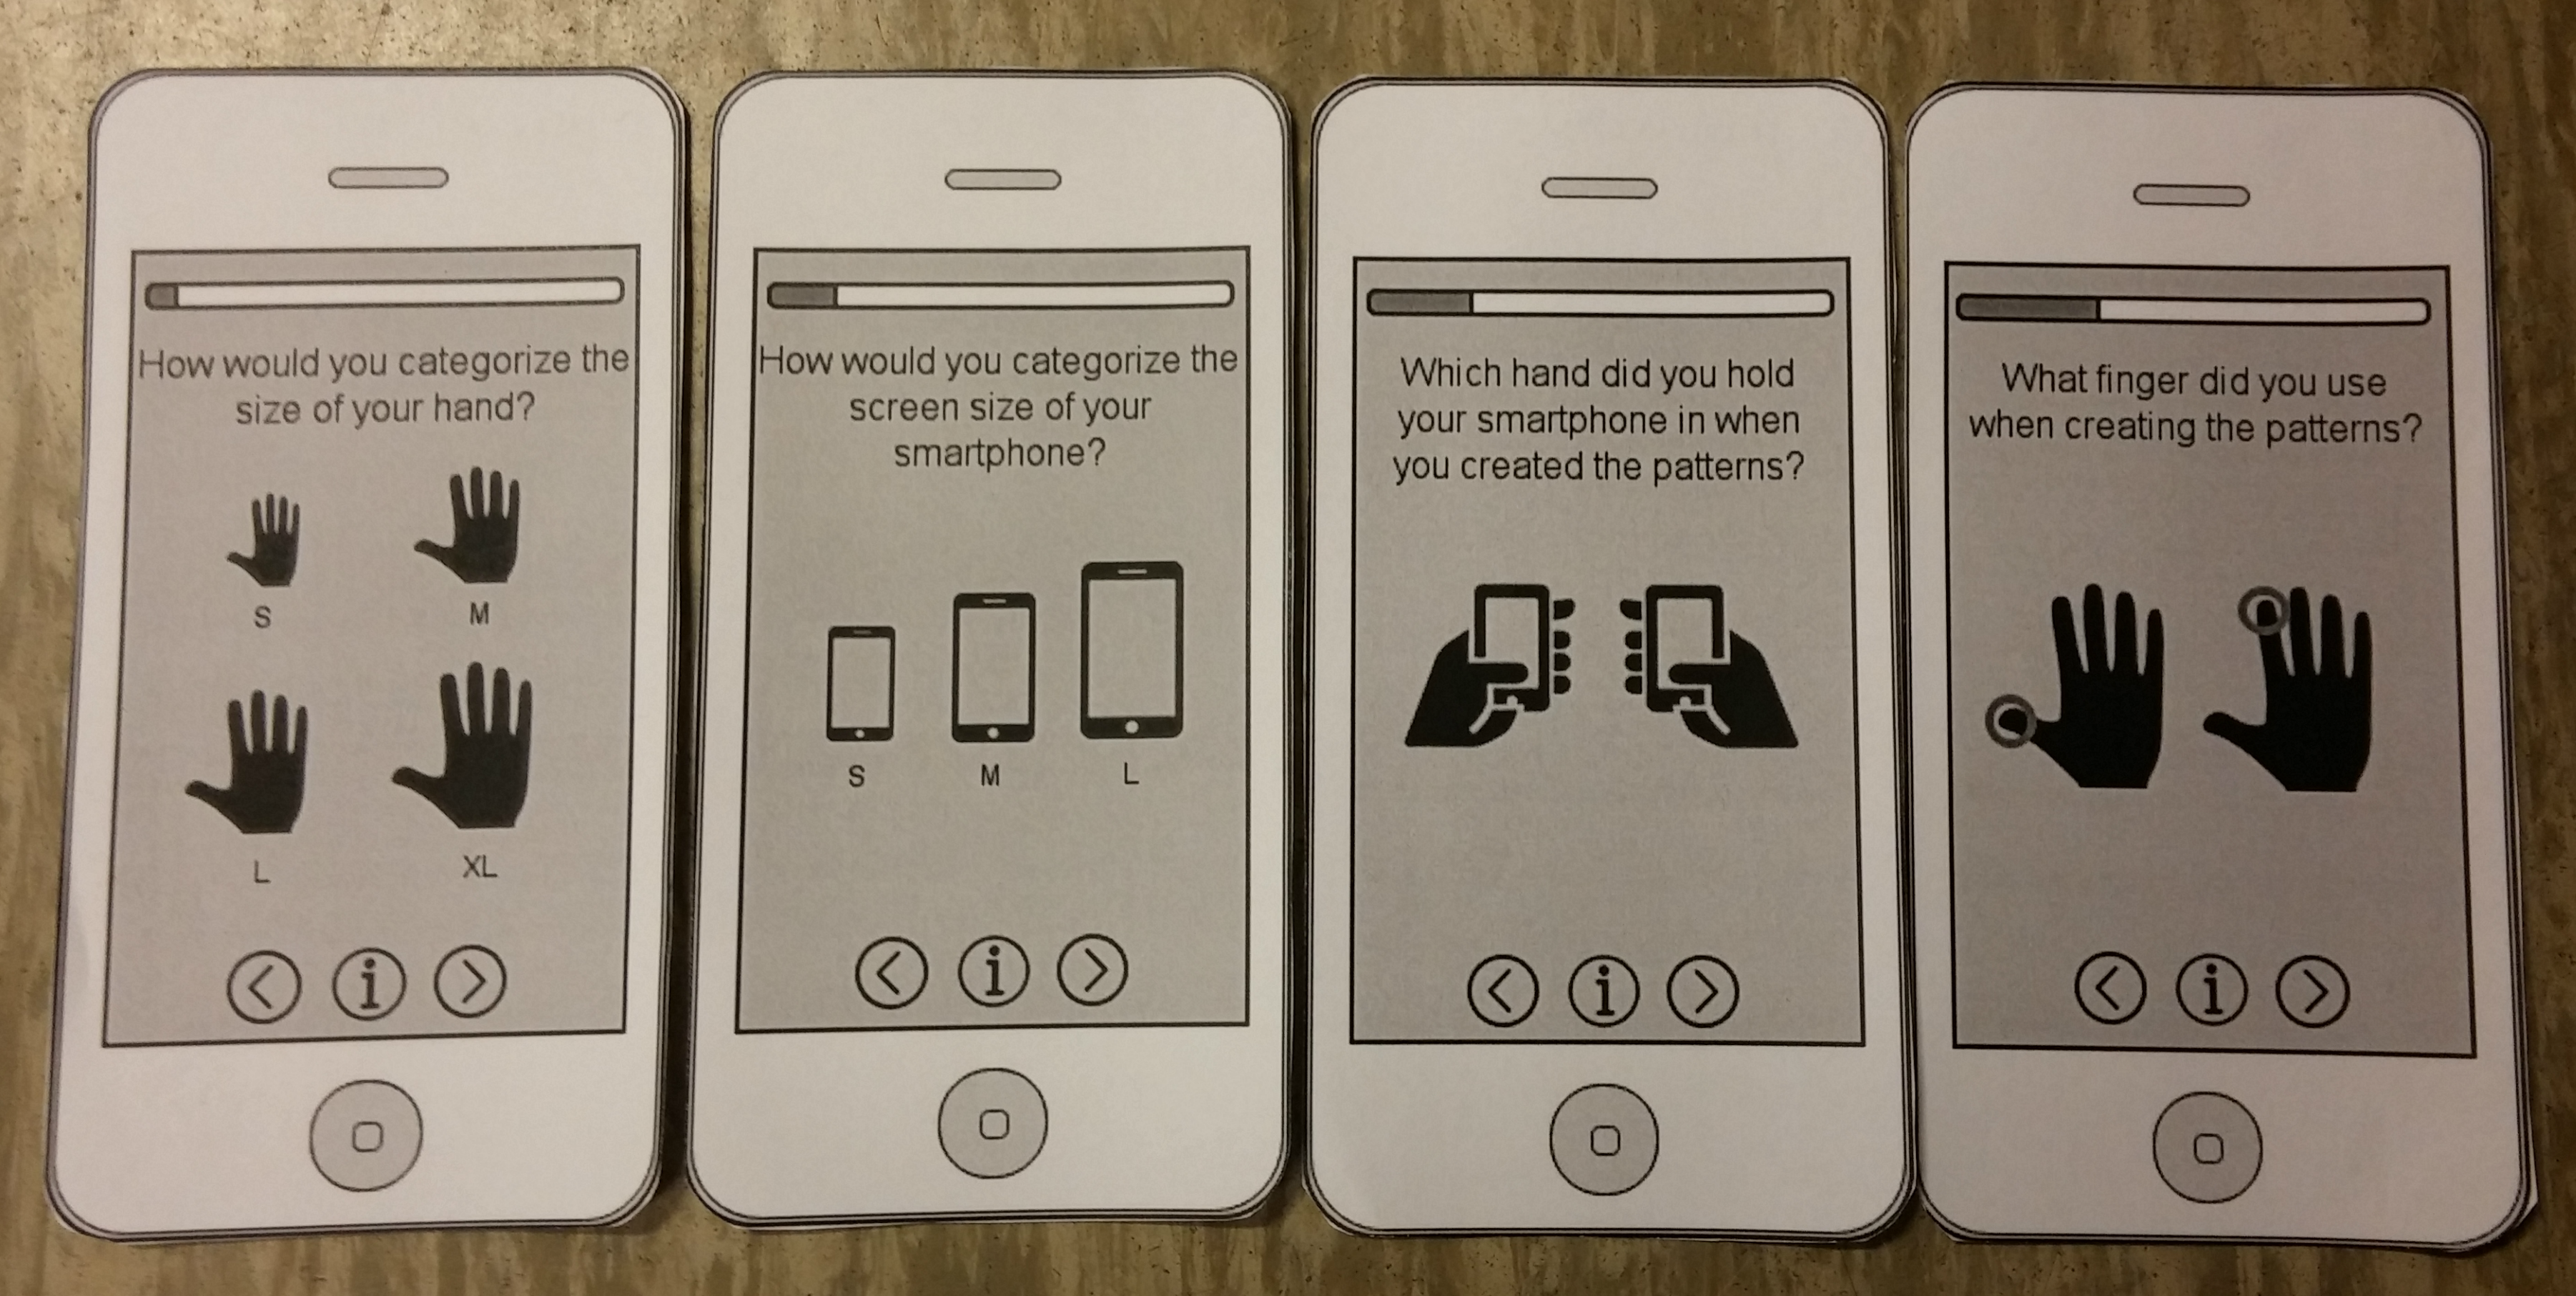
\includegraphics[scale=0.08]{pics/test1.png}
      \caption{Usability test 1}
      \label{fig:test1}
    \end{figure}

  In the second test, it only tested the effectiveness (measured in number of errors) by only looking at the icons. When showing the icons to the participant, the actual question was covered. The students that participated in the test was supposed to guess what was asked for and select their answer by only looking at the icons. When conducting this test, the goal was to be able to see if the icons was understandable. When sending out the questionnaire, it is important that respondent that are not fluent in English are able to answer the questions without be able to understand all the English words. It is also useful for respondents to be able to use the text and the icons together in order to understand the questions. Figure~\ref{fig:test2} is showing an image from test 2, where the question is covered. 

    \begin{figure}[H]
      \centering
      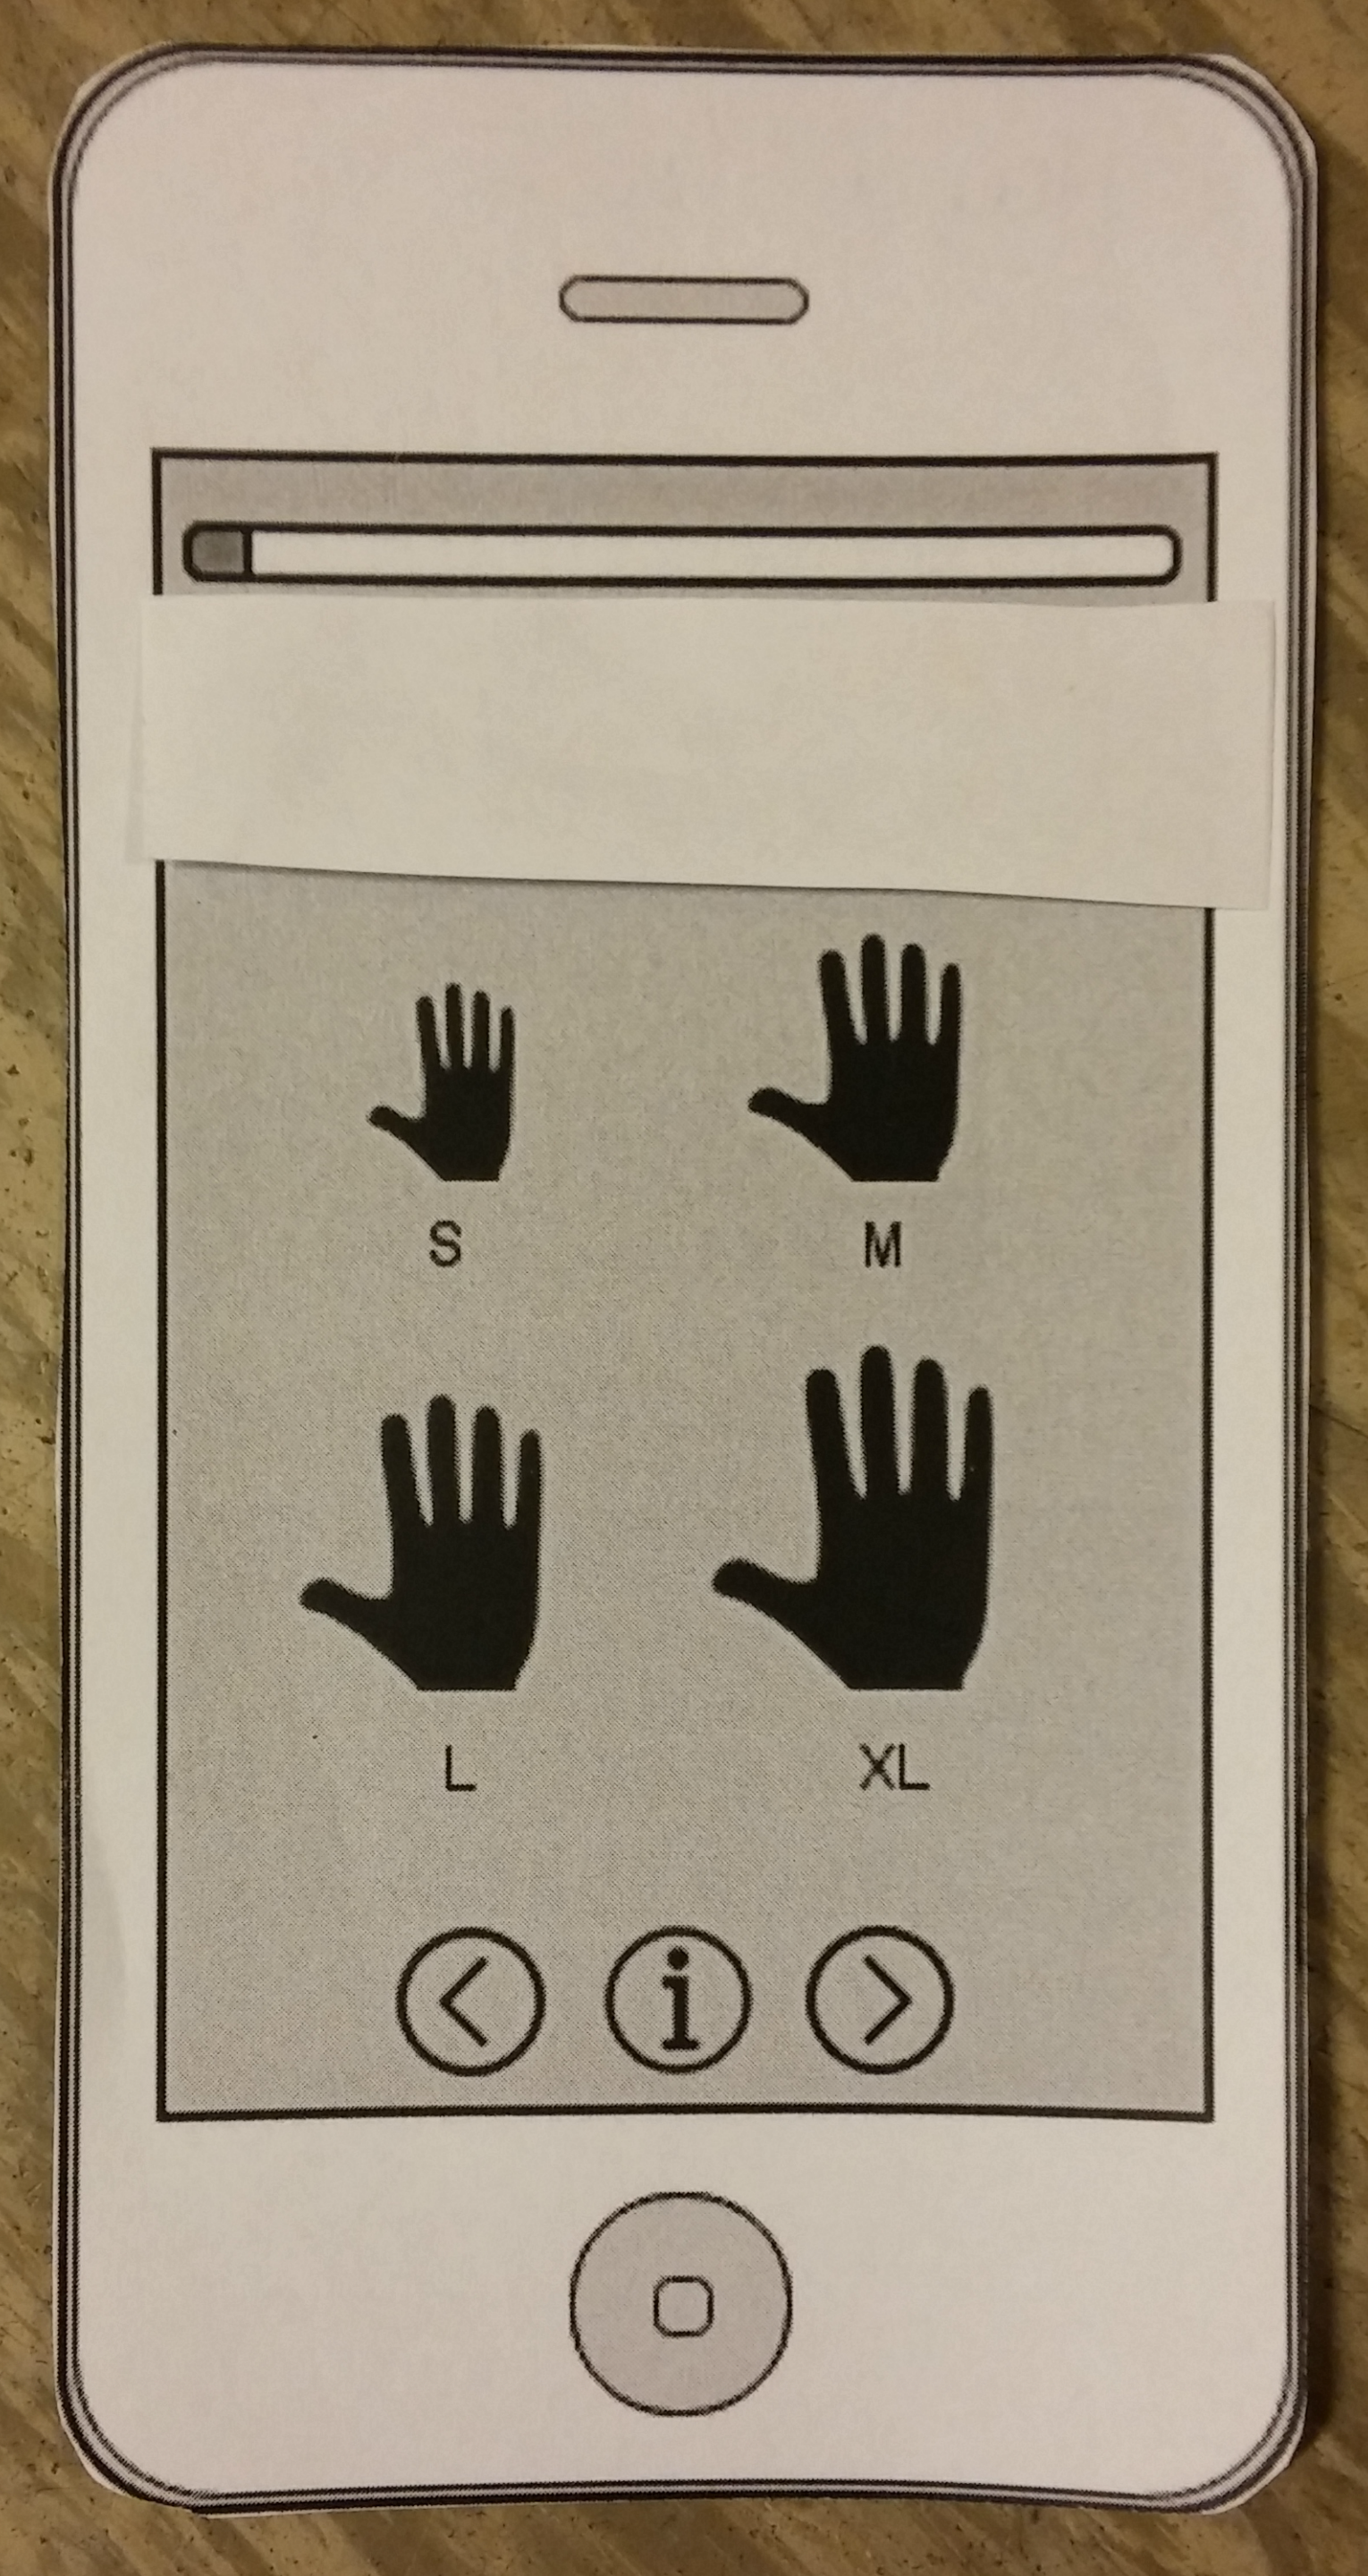
\includegraphics[scale=0.05]{pics/test2.png}
      \caption{Usability test 2}
      \label{fig:test2}
    \end{figure}

  \subsubsection*{Results}

  For testing the prototype I contacted 5 girls and 5 boys (age from 20-24) from the university, resulting in 5 participants for each test. This is a small number of participants, and is not representing the whole population. The main goal was to get some feedback on the wireframes from Section~\ref{fig:wireframes}. The feedback from the participants will be included in the next version of the prototype. The new prototype will be tested an implemented next semester. 

  In test 1, all the wireframes was used, and was demonstrated in the same order as Figure~\ref{fig:wireframes}. The participants were explained that the test did not test their knowledge, rather the systems and its design. If they ever felt uncomfortable, they were also explained that they could quit the test whenever they wanted. Before they started on the questionnaire, they were given information about the research, their right to stay anonymous, and the purpose of the research. The participants started when they pressed ``Start'' as illustrated in Figure~\ref{fig:wireframe1}. During the test the participants commented on some part of the test.

  {\bf Comment on Figure~\ref{fig:wireframe20}}: {\it I study, but I have not finished my studies. Should I press yes?}. All of the respondents was unsure whether to select yes or no on the question about their experience with IT and security. All the participants were IT-students, and all was unsure if the word ``studied'' was fitting their situation since they still were students. Most of the students chose to select ``no'' as their answers, but I would probably categorize all of them in a group that have experience with IT and/or security. This question should be redesigned in order to avoid respondents to get in the same position. 

  {\bf Comment on Figure~\ref{fig:wireframe12}}: ``What is a do you mean by reading and writing orientation?''. One of the students were unsure what this question asked for. The student guessed that the question asked for the direction that he used to write, but he got unsure when he red the alternative ``top-to-bottom'' because that alternative didn't relate to him. He then clicked on the information button, and I explained what the different reading orientation was.



  After the participants completed the question, I asked a set questions:

  \begin{itemize}
    \item 
  \end{itemize}

  In test 2, the respondents was challenged with the wireframes that contained icons. They guessed what was asked for and then selected they answer with an explanation of why they did so. All the five respondents (three girls and two boys) managed to interpret the icons and guess most of the questions. 
  There was one participant that guessed that wireframe~\ref{fig:wireframe16} was asking if they used the Android scheme. It is quite close, but not the exact question. I don't see this as a problem because all the respondents from test 1 manage to interpret the question correctly.

  \subsubsection*{Redesign}

  Navigation

  \subsection{Validity and Reliability}\label{sec:validityandreliability}

    {\bf Content validity}

    {\bf Construct validity}

    {\bf Reliability}
	\section{Ethical Considerations}
\label{sec:ethical}

	In this section the ethics of this research will be discussed. My research is done by collecting demographics and personal data, as well as asking the respondents to enter a password. Before doing research it is important to look into the ethical aspects to see if the data collected is legal and protect the personal data being anonymous. 

	Before the questionnaire starts, the respondents are informed about the purpose of the research and how their contributed data will be used. Respondents also must be informed that they have the right not to participate. The questionnaire should be fully anonymous and their identity and location are not possible to track. 

	The demographic information collected do not provide any information that make it possible to track the data back to the respondent. 

	% Chapter 5 - Further Work
	\chapter{Future Work} \label{chap:FutureWork}

	This chapter will provide a suggestion for future work when continuing on this research next semester.

\section{Redesign of Prototype}
  
  The prototype still needs to be worked on. After conducting the usability tests, I got some new suggestion for improvements:

	{\bf Navigation}: When implementing the system, it is a need to look at the navigation in a different way. In the usability test, all the participants would like a faster way of navigation between the questions asked. One of the proposed solutions is to go automatically to the next questions with support for going back if they selected a wrong answer.

	{\bf The order of the patterns:} One of the respondents requested that it be preferable that the mobile pattern was asked for first because that was a known environment for her. In the design it is stated that is preferable to give a random order of the patterns (using a Latin Square) in order to be able to see if the ordering is impacting the way the respondents create their patterns. This needs to be looked further into when implementing the system. If would be preferable to test whether it will give a higher level of real world data when asking for the mobile patterns first.

	{\bf Icons used:} The wireframes included icons that were found on the web, and some of the icons might need to be resigned in order to illustrate its corresponding value in a better way. One example is one of the alternatives in Figure~\ref{fig:wireframe18} that is trying to illustrate the ``slide-to-unlock'' locking mechanism (the second icon on the right side).

	Besides the navigation and the order of the patterns, there was not provided any other feedback that needs to be redesigned before the implementation. The first version of the implemented system needs to go through a new usability test before starting the actual data collection.

	\section{Implementation of Prototype}

	The prototype is still not implemented, and it needs to be finished before I am able to start collecting data. I need to decide what kind of technologies that I want to use. After implementing the system, I should conduct a new usability test as described in the last chapter. One change would be to test the system on an actual smartphone, and not on paper. The results of a test would be more accurate when using the real environment of the system. The test will provide feedback on improvements before sending out the questionnaire.

	\section{Data Collection Permission}

	Before collecting data, it is required to ask for permission to do so from ``Personvernombudet for forskning''(NSD) \cite{personvernombud}. NSD is the privacy ombudsman for approximately 150 research and educational institutions in Norway, where NTNU is one of them. The data collection can start when I have granted allowance from NSD to conduct the data collection.

	%Bibtex
	\bibliographystyle{plain}
	\bibliography{myBib}
	
\end{document}